
\section*{Problema P7.53}

\renewcommand*\thesection{7.53}
\numberwithin{equation}{section}
\numberwithin{figure}{section}

\begin{center}
    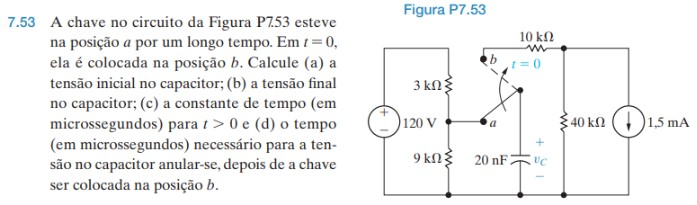
\includegraphics[scale=1.0]{P7.53.jpg}
\end{center}

\subsection*{(a)}

Em $t<0$, como o capacitor está em paralelo com um divisor de tensão, a tensão inicial no capacitor é dada por  

\[ v(0) = 120\frac{9\un{k}}{3\un{k} + 9\un{k}}  \]

\[ \boxed{v(0) = 90 \un{V}}  \]

\subsection*{(b)}

Vamos determinar a função da tensão no capacitor para $t>0$. Usando transformações de fonte,
podemos reduzir o circuito com a chave na posição $b$ para o circuito da Figura \ref*{fig:7.53.1}.

\begin{figure}[hb]
    \centering
    \caption{Circuito com a chave em $b$ reduzido.}
      \centering
      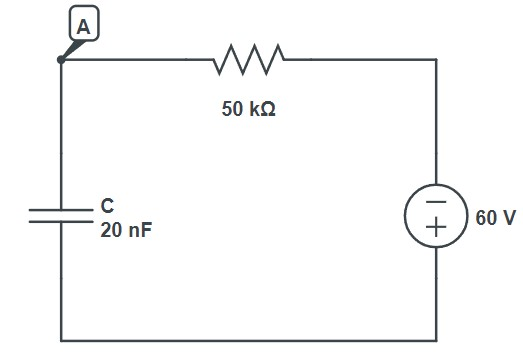
\includegraphics[scale=0.5]{P7.53-Item(b).jpg} \\
    \label{fig:7.53.1}
\end{figure}

Feito isso, aplicamos análise nodal no nó (A) mostrado em \ref*{fig:7.53.1}.

\[ -i_c + \frac{V_A - (-60)}{50\un{k}} = 0  \]

Usando $V_A = v$, $i_c = C\diff{v}{t}$ (com a convenção passiva), temos

\[ -(-C\diff{v}{t}) + \frac{v}{50\un{k}} = - 12 \cdot 10^{-3} \]

\[\diff{v}{t} + \frac{v}{C50\un{k}} = - \frac{12 \cdot 10^{-3}}{C} \]

\[ \diff{v}{t} + \frac{v}{0.001} = -60000 \]

Usando o fator integrante $M(t) = e^{1000t}$,

\[ e^{1000t}\diff{v}{t} + e^{1000t}\frac{v}{0.001} = -60000 e^{1000t} \]

Aplicando o inverso da regra da derivada do produto,

\[ \diff{[v(t) \cdot e^{1000t}]}{t} = -60000 e^{1000t} \]

\[ v(t) \cdot e^{1000t} = \int -60000 e^{1000t} \, dt \]

\[ v(t) = e^{-1000t} (-60000) \frac{1}{1000} [ e^{1000t} + K ] \]

\[ v(t) = - 60 - 60Ke^{-1000t} \]

Sabemos que, do item (a), $v(0) = 90 \un{V}$, logo temos $K = -2.5$ e 

\begin{equation}\label{eq:7.53.1}
    v(t) = - 60 + 150 e^{-1000t} \un{V} \, , \, t \geq 0
\end{equation}

Uma vez determinado a função de $v(t)$, temos que valor final $v(\infty)$ da tensão é    

\[ \displaystyle \lim_{t\to \infty} v(t) = -60 + 0 = - 60 \un{V}  \]

\[ \boxed{v(\infty) = - 60 \un{V}} \]

\subsection*{(c)}

Na expressão de $v(t)$ encontrada em \eqref{eq:7.53.1}, temos 

\[ \boxed{ \tau = \frac{1}{1000} = 1 \un{ms}} \]

\subsection*{(d)}

Isolando $t$ em \eqref{eq:7.53.1}, temos 

\[ e^{-1000t} = \frac{v(t) + 60}{150} \]

\[ -1000t = \ln\left(\frac{v(t) + 60}{150}\right)  \]

\[ t = -\frac{1}{1000} \ln\left(\frac{v(t) + 60}{150}\right)  \]

Queremos o instante $t$ tal que $v(t) = 0$. Substituindo $v(t) = 0$ na expressão acima, temos

\[ t = -\frac{1}{1000} \ln\left(\frac{60}{150}\right)  \]

\[ \boxed{ t = 916.29 \un{$\mu$s}} \]





